In the framework of N3, the discrimination of the SOM in \textit{fanaux} can be carried out by hierarchical ascending classification -- noted CAH -- according to the Ward's method. The choice of the method remains empirical, but this appears the most appropriate within the framework of an automatic classification.

\bigskip

Here are some lineaments of the CAH and the Ward's method, which are described more precisely in the articles \textit{The automatic classification of quantitative data} \citep{mc} and \textit{Distances between Clustering, Hierarchical Clustering} \citep{cs}.

\begin{figure}[htbp]
\begin{center}
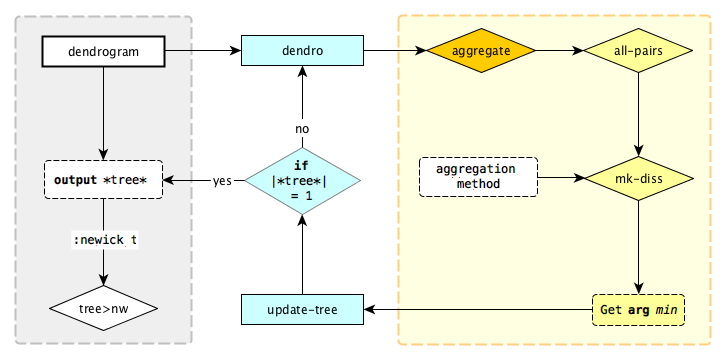
\includegraphics[width=\columnwidth]{2341}
\caption{Diagram of the CAH algorithm of \glspl{dendrogram}.}
\label{fig:cah}
\end{center}
\end{figure}

Note that \glspl{dendrogram} generates a newick\footnote{To know more about the Newick tree format see the Web page description by Joseph Felsenstein and by Gary Olsen at:\\ \indent \href{http://evolution.genetics.washington.edu/phylip/newicktree.html}{\texttt{\scriptsize http://evolution.genetics.washington.edu/phylip/newicktree.html}}} file by default allowing to display or else the tree with a third-party application.

%\bigskip
%\bigskip
\newpage

\noindent {\large \textbf{Ward's method}}

\bigskip

With the Ward's method, the distance between two classes $A$ and $B$ is computed as follow:

$$d(A,B)=\frac{|A||B|}{|A|+|B|}d(g_{A}, g_{B})^2$$

with the mean value:

$$g_{\mathcal{P}}=\frac{1}{|\mathcal{P}|}\sum_{i \in \mathcal{P}}s_i=\overline{x}$$


In some case, the dendrogram hierarchy may have inversions. This can be avoided by applying the following relation: 

$$\forall A, B \in H, h (A \cup B) = max (d (A, B), h (A), h (B))$$

\bigskip

%\newpage

Finally, the intraclass inertia is computed for each node as a potential class $C$ such that:

$$I_C=\frac{1}{|C|}\sum_{e \in C}d(e,g_C)^2$$